\documentclass[UTF8]{article}
    \usepackage{graphicx} 
    \usepackage{fontspec,xunicode,xltxtra}
    \usepackage{titlesec}
    \usepackage[top=1in,bottom=1in,left=1.25in,right=1.25in]{geometry} 
    \usepackage{indentfirst}             % 段首缩进
    
    \setmainfont[BoldFont=SimHei]{SimSun}% 默认字体为宋体
    
    \XeTeXlinebreaklocale "zh"           % 中文断行
    
    \newfontfamily\kai{STKaiti}          % 楷体
    \newfontfamily\hei{SimHei}           % 黑体

    \begin{document}
        \section{编译器简介}
        test编译器将某种语言转化为另一种程序.源语言通常是C/C++,Java等,目标语言通常是处理器的指令集.\par    
        \begin{figure}[h]    
            \centering    
            
\includegraphics{chapter1_1.eps}   
            \caption{编译器}    
            \label{Fig 1}    
        \end{figure} 
        编译器的基本原则:\par
        \kai{
            编译器必须保持被编译程序的语义.\par
            编译器必须以某种可觉察的方式改进输入程序.\par
            }
        \begin{figure}[h]     
            \centering    
            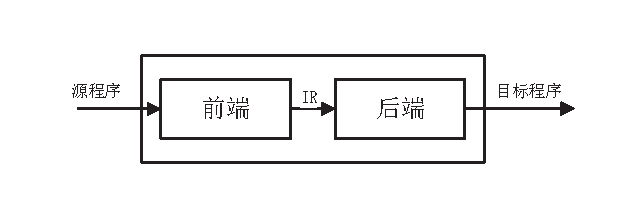
\includegraphics{chapter1_2.eps}   
            \caption{IR}    
            \label{Fig 2}    
        \end{figure} 
        \emph{编译器使用一些数据结构来表示它处理的代码,这种形式称为中间表示(intermediate representatition,IR)}\par
        
        \emph{优化器:\par
            编译器中间的部分叫做优化器,负责简化IR.
        }\par

        
    \end{document}